\section{First images from the Light Microscopy Module (LMM)}\label{first-images-from-the-light-microscopy-module-lmm}
We have 15 samples in the holder in this set of experiments, and our first task
is to image all of the samples with the lowest-magnification microscope
objective lens (2.5x). This lens's magnification is ideal for the task, as it
gives an image of each entire sample well. We first use brightfield transmission
illumination (50/50 filter), where the intensity of the image is proportional to
the amount of light passing through different parts of the sample. Thus,
magnetic stir bar appears dark, as it transmits no light, and the glass appears
bright, as most of the light passes through. Bubbles act as mini-lenses, and
therefore are bright in the center and dark around their edges; the light from
the edges is bent toward the center (or focused) by the bubble. These features
are evident in an image of well number 5, containing a phase-separating sample,
as shown in the image on the left.
\begin{figure}
\begin{center}
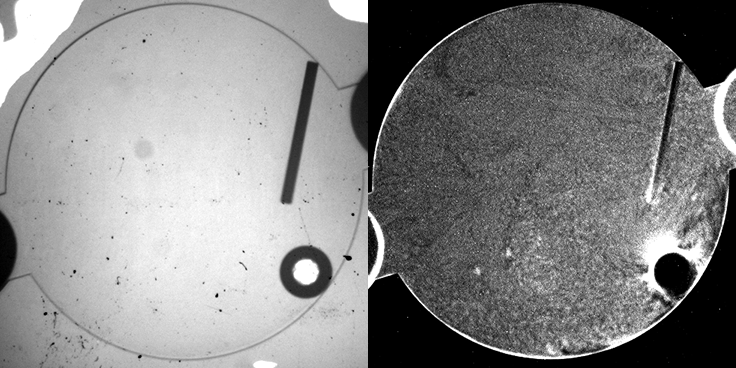
\includegraphics[width=\columnwidth]{./images/2014_06_04_first_day/140604_well5_2p5x.png}
\caption{well 5, 2.5x mag, brightfield transmission}
\end{center}
\end{figure}

The image on the right is the same sample and position, but collected in
fluorescence mode, where the intensity is proportional to the number of
(fluorescent particles). Interestingly, we observe higher concentrations of
particles aggregating around the edges of the sample chamber, the stir bar and
the bubbles. Neither the stir bar nor bubble contain any fluorescent particles,
and like the background glass appear black.

\section{Compositing images to get a higher-magnification view of the entire sample}\label{compositing-images-to-get-a-higher-magnification-view-of-the-entire-sample}
The 2.5x images are good to show the entire sample, but the resolution is
limited. To get a higher-resolution view of the sample, we switch to a
higher-magnification objective lens; however, the tradeoff is that the field of
view is curtailed, and only part of the sample fits into the visible field of
view. Fortunately, the LMM has an automated stage, so that the position of the
sample visible to the microscope can be controlled remotely. As a result, we can
take images in a tile-pattern that cover the entire sample:

\begin{figure}
\begin{center}
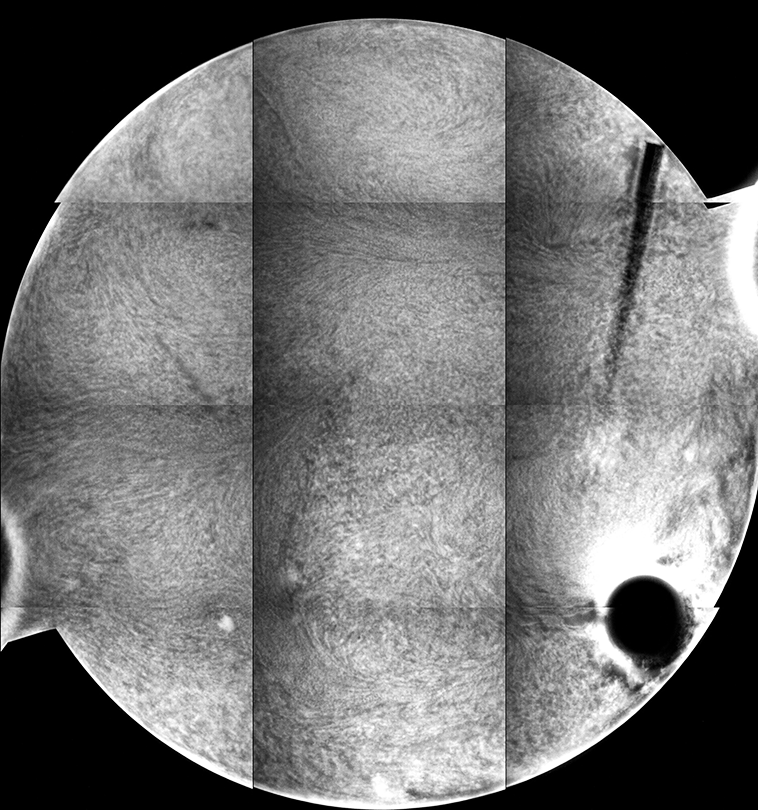
\includegraphics[width=\columnwidth]{./images/2014_06_04_first_day/140604_well5_composite}
\caption{well 5, 10x mag, fluorescence tiled composite}
\end{center}
\end{figure}

The different fluorescence images are the tiled composite image taken at
different depths from the cover slip inside the sample. If you look at the stir
bar, you can see how different parts of the bar come into ``focus'' in the
different images, giving an indicator of the depth within the sample from which
the images are collected.

Each ``tile'' is a bit darker to the left, so that the rectangles representing
each individual 10x image are easily seen. This is a result of uneven
illumination; the samples are illuminated by light from a lamp, which does not
cover the sample evenly (which might be ameliorated by changing internal
microscope aperture settings).

But we have another way we might correct for this problem: a couple of our
samples are fluorescent dye dispersed in a solvent inside identical sample
wells---physically, the intensity of fluorescence should be completely even /
isotropic, so any unevenness in the image should be caused by the illumination.
By taking images under identical conditions of both the phase-separating sample
of interest, and of the even dye solution, we should be able to cancel the
background and see the sample without the effects of the uneven lamp
illumination. So we will be testing this in upcoming operations.

Meanwhile, next stage is to look at higher-magnification, where we seek to
understand the details of small portions of the sample, and see the behavior of
these colloid structures up close.